\documentclass{beamer}
%\documentclass[handout]{beamer}

\usepackage{pgfpages} 
%\pgfpagesuselayout{4 on 1}[letterpaper,border shrink=5mm,landscape] 
%\pgfpagesuselayout{2 on 1}[letterpaper,border shrink=2mm]

\usetheme{default}

\mode<presentation> {
%  \usetheme{Warsaw}
  \usetheme{Frankfurt}
%  \usetheme{Boadilla}
%  \usetheme{Marburg}
}

\mode<handout>{\setbeamercolor{background canvas}{bg=black!5} %
    \pgfpagesuselayout{2 on 1}[letterpaper,border shrink=4mm] }

\title[Bighouse Crash] {A Crash course to (The) Bighouse}
\author{Brock Palen\\ \texttt{brockp@umich.edu}}
\date{SVTI Users meeting Sep 20th}

\begin{document}
  \setbeamercovered{transparent}  
  \begin{frame}
    \titlepage
  \end{frame}

%table of contents
  \begin{frame}{Outline}
    \tableofcontents
  \end{frame}
  
  \section{Resources}
  \subsection {Configuration}
%bighouse
  \begin{frame}{Hardware: bighouse}
   \begin{columns}[c]
    \begin{column}{7cm}
    \begin{block}{Bighouse}
    \begin{itemize}
      \item bighouse is our Itanium SMP machine;
      \item Login: \texttt{bighouse.engin.umich.edu}
      \item Shares nyx's 6TB NFS file system
      \item Running SUsE Linux Enterprise Server 10
      \item ProPack 5 from SGI
    \end{itemize}
   \end{block}
   \end{column}
   \begin{column}{5cm}
    \begin{center}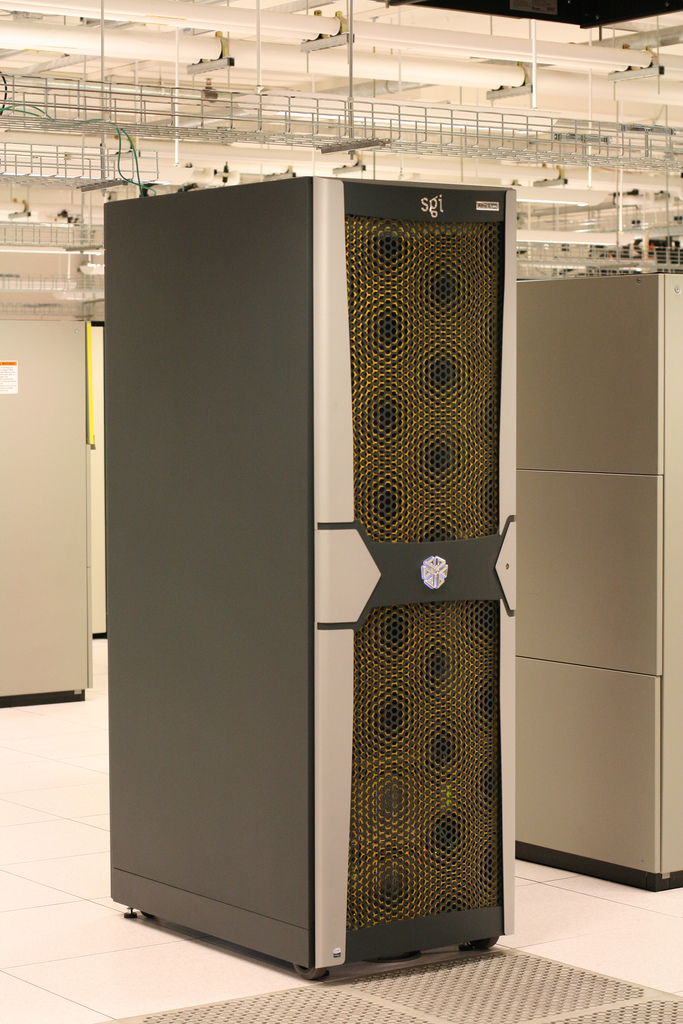
\includegraphics[height=2.7in]{tallbighouse}\end{center}
   \end{column}
   \end{columns}
  \end{frame}
%arch
  \subsection {Hardware}
  \begin{frame}{Bighouse Hardware}
   \begin{block}{Current Hardware}
   \begin{itemize}
    \item<2->16 CPU, 32 core Intel Itanium II's
    \item<3->Measured 5.5 Gflop/cpu running 4 way
    \item<3->171.9 Gflop running 32 way
    \item<4->96 GB Ram
    \item<5->Max 41 GB/s Aggregate Memory bandwidth
   \end{itemize}
   \end{block}
  \end{frame}

  \section{Architecture}
  \subsection{ccNUMA}
  \begin{frame}{ccNUMA}
   \begin{center}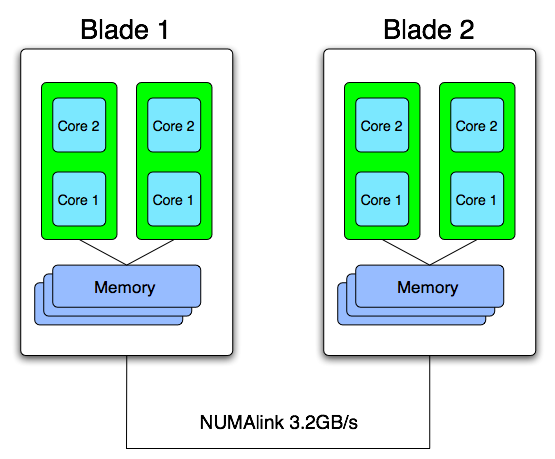
\includegraphics[height=2.5in]{numa}\end{center}
  \end{frame}
  \subsection{Altix 4700 Brick}
  \begin{frame}{Altix 4700 Brick}
   \begin{center}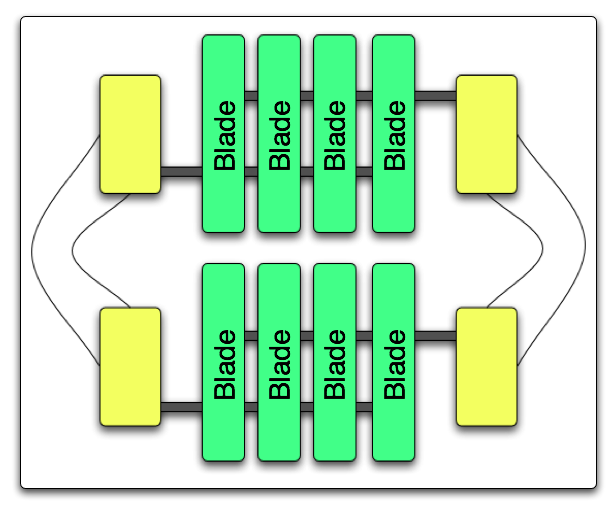
\includegraphics[height=2.5in]{bighouseBrick}\end{center}
  \end{frame}

\section{Software}
\subsection{Packaged Software}
\begin{frame}{Packaged Software}
\begin{block}{Packaged Software}
 \begin{itemize}
  \item<1>{Abaqus/6.6}
  \begin{itemize}
   \item{\texttt{abaqus\_v6.env}}
   \item{\texttt{standard\_memory\_policy=15000mb}}
   \item{\texttt{standard\_memory\_policy=MAXIMUM}}
  \end{itemize}
  \item<2>{Nastran/2007r2}
  \item<3->{Gaussian/03}
  \begin{itemize}
   \item{\texttt{\%nproc=8}}
   \item{\texttt{\%mem=20gb}}
   \item<4->{\alert{DO NOT SET \texttt{\$GAUSS\_SCR}}}
  \end{itemize}
 \end{itemize}
\end{block}
\end{frame}
\begin{frame}{Abaqus}
\begin{block}{Abaqus Example}
  \begin{itemize}[<+-| alert@+>]
   \item{\texttt{mkdir /tmp/\$PBS\_JOBID}}
   \item{\texttt{cd /tmp/\$PBS\_JOBID}}
   \item{\texttt{cp \~{}/Input.inp .}}
   \item{\texttt{cp \~{}/abaqus\_v6.env .}}
   \item{\texttt{abaqus job=Input scratch=/tmp interactive cpus=10}}
   \item{\texttt{cp -fr * \~{}/ \&\& rm -fr /tmp/\$PBS\_JOBID}}
  \end{itemize}
\end{block}
\end{frame}
\begin{frame}{Nastran}
\begin{block}{Nastran Example}
  \begin{itemize}[<+-| alert@+>]
   \item{\texttt{mkdir /tmp/\$PBS\_JOBID}}
   \item{\texttt{cd /tmp/\$PBS\_JOBID}}
   \item{\texttt{cp \~{}/Input.inp .}}
   \item{\texttt{cp \~{}/abaqus\_v6.env .}}
   \item{\texttt{nastran batch=no hpmpi=yes dmp=10 input.dat}}
   \item{\texttt{cp -fr * \~{}/ \&\& rm -fr /tmp/\$PBS\_JOBID}}
 \end{itemize}
\end{block}
\end{frame}

\subsection{Compiled Code}
\begin{frame}{Compilers}
 \begin{block}{Compilers}
  \begin{itemize}
   \item<1->{\texttt{ifort} Fortran90/77}
   \item<1->{\texttt{icc} C }
   \item<1->{\texttt{icpc} C++}
   \item<2->{GNU Compilers are available but not recommended}
  \end{itemize}
 \end{block}
 \begin{block}{Compiler Options}
  \begin{itemize}
   \item<3->{\texttt{-O2} General optimization}
   \item<3->{\texttt{-O3 -ipo -funroll-loops -ftz} Better Optimization}
   \item<3->{\texttt{-openmp} Enable OpenMP support}
  \end{itemize}
 \end{block}
\end{frame}
\begin{frame}{Libraries}
 \begin{block}{Libraries}
  \begin{itemize}
   \item<1->{MPT}
   \begin{itemize}
    \item<1->{MPI Library Optimized for Shared Memory}
    \item<2->{\texttt{ifort source.f90 -lmpi}}
    \item<2->{\texttt{mpirun -np 10 a.out}}
   \end{itemize}
   \item<3->{MKL Math Kernel Library}
    \begin{itemize}
     \item{Optimized Threaded Math Library}
     \item{Full Support for BLAS and LAPACK}
     \item{PRNG FFT's, and FFTW compatible}
     \item{\alert{DO} Use, Contact us for support}
    \end{itemize}
  \end{itemize}
 \end{block}

\end{frame}

\section{PBS}
\subsection{PBS Queues}
\begin{frame}{PBS}
\begin{block}{PBS}
 \begin{itemize}
  \item{Memory is Enforced}
  \begin{itemize}
   \item{Defaults to 1MB}
   \item{Use \texttt{\#PBS -l mem=100mb} to request what you need}
  \end{itemize}
  \item{Use \texttt{route} queue}
  \item{Only 30 cpus available for batch jobs}
  \item{2 cpus for compiling sftp PBS etc}
  \item{Please clean up \texttt{/tmp}}
 \end{itemize}
\end{block}
\end{frame}
\begin{frame}{Questions}
 \begin{block}{Questions?}
 Questions?
 \url{http://cac.engin.umich.edu/resources/bighouse.html}
 \url{cac-support@umich.edu}
 \end{block}
\end{frame}
\end{document}
